\section{Results}
\begin{marginfigure}
	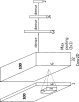
\includegraphics[width=1\marginparwidth]{imu-cnn-korrekt}
	\caption[Model architecture]{Model architecture of the neural network of general models for predicting touches based on phones' IMU.}
	\label{fig:model_architecture}
\end{marginfigure}
\subsection{Data Set \& Preprocessing}
\label{sec:prepro}

We recorded a total of 1079 minutes of sensor data from the \textit{touch} and \textit{Fitt's Law task} task.
The duration for touches was on average 664.56ms (SD = 300.69ms).
The fastest touch was performed within 181ms.
%Since we are only interested in sensor changes during the process of reaching for a target and touching it and the purpose of the \textit{Fitt's Law task} was only for reseting the participants grip to the lower half of the phone our first step in our preprocessing pipeline was \texttt{cutting} out the sensor fragments of the \textit{Fitt's Law task}.
During the study we sampled the linear accelerometer, gyroscope, magnetometer, gravitational sensor, and the orientation sensor.
Due to the high sampling rate of the sensors we first removed occurring duplicates by keeping the last sensor value and timestamp.
We then up-sampled the sensors to 333.33 Hz, resulting in 1 sample given every 3ms. 
Finally, we saved 100 samples before each touch resulting in a total of 3.456.000 samples.
After testing we only kept the accelerometer and the gyroscope, as using all sensors led to overfitting.

Up-sampling the sensors to 1 sample every 3ms resulted in a discontinuous function for each sensor axis. 
We have therefore tried applying several smoothing procedures, including a Butterworth lowpass-filter and a moving average filter.
Both approaches, however, did not lead to an increase in accuracy, so we have adhered to the unsmoothed data of the sensors.

\subsection{Baseline}
We explored basic regressors from scikit-learn \footnote{\url{https://scikit-learn.org/stable/supervised\_learning.html\#supervised-learning}} as a baseline to test whether using novel machine learning techniques is sufficient for touch prediction with IMU.
The used regressors are abbreviated as follows: RandomForestRegressor (RF), Decision Tree Regressor (DT), K Nearest Neighbors Regressor (KNN), and Gaussian Processes Regressor (GP).
We performed a grid search for the different regressors to find the best hyperparameters for each regressor.
The results for all phones with different time configurations of all regressors can be seen in \cref{tab:baseline}.
Light green highlighted values in phone columns represent the regressor that performed the best for this configuration of phone and prediction time.
Green highlighted values in the first column represent the overall best regressor for each prediction time.

\subsection{Neural Network}

We implemented our neural network using \textit{Keras} 2.2.4 which is based on the TensorFlow backend.
We trained two model types, one which we call \textit{single} and one which we call \textit{general} model.
Single models were trained on sensor and touch data of single phones; general models were trained on sensor data and normalized touch data of all phones.
\begin{marginfigure}	
	\centering
	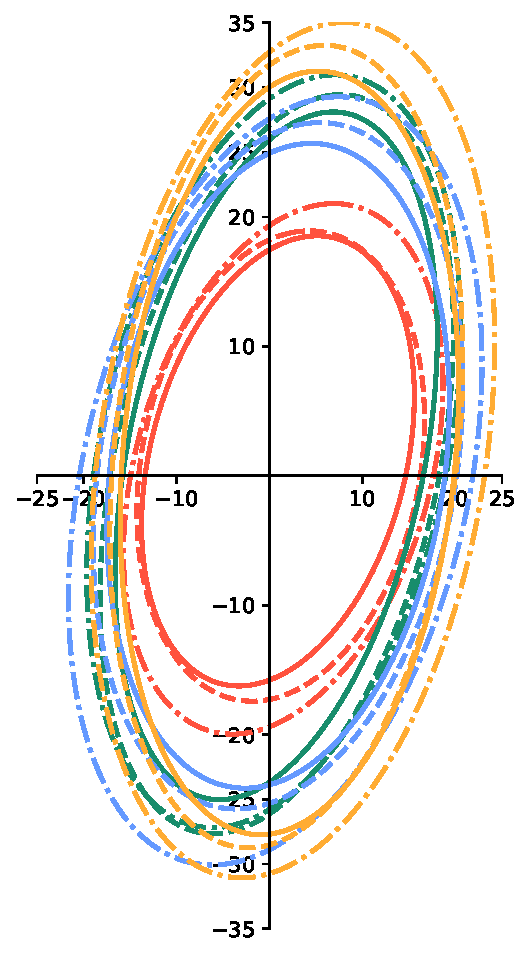
\includegraphics[height=\linewidth]{ellipses_single}
	\caption{Elliptic envelope plot for single models.\newline}
	\label{fig:ell_single}
\end{marginfigure}
\begin{marginfigure}
	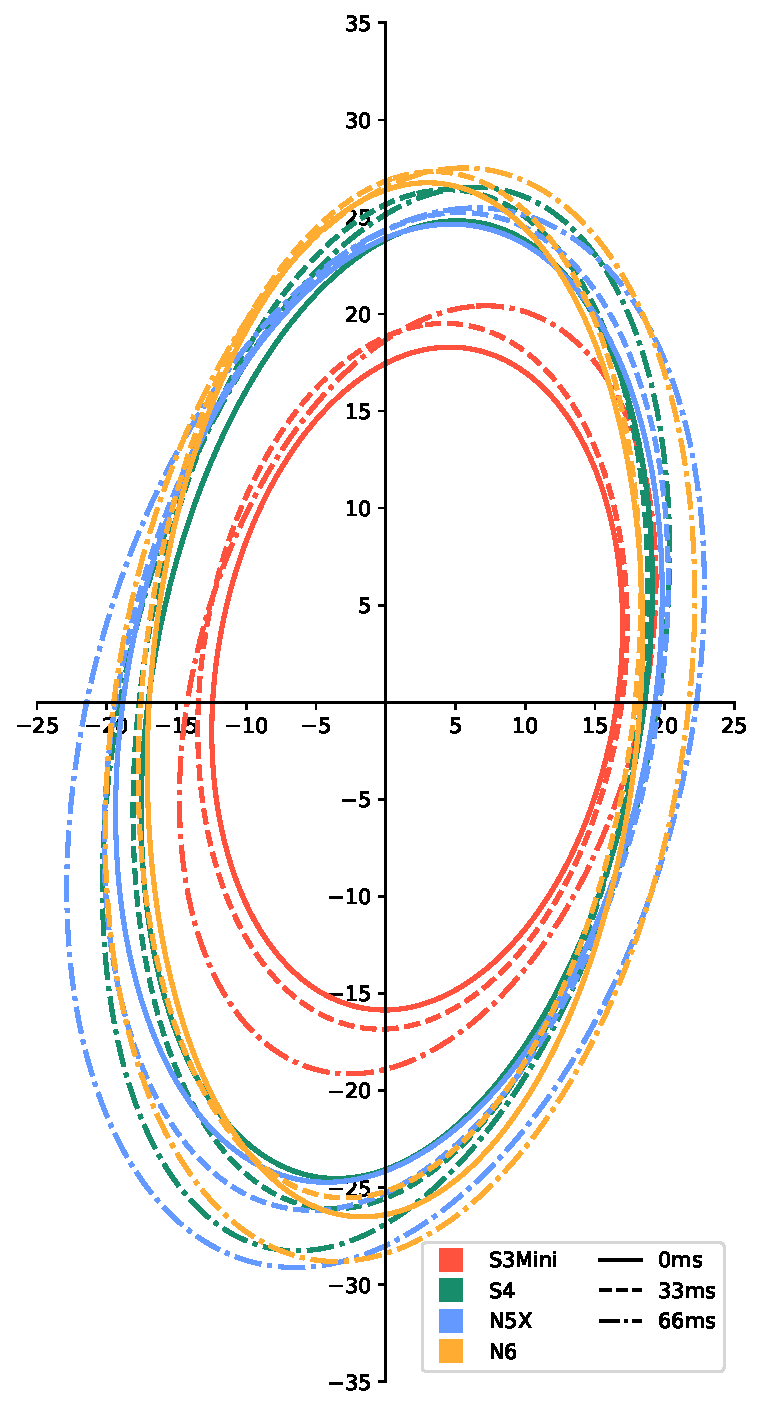
\includegraphics[height=\linewidth]{ellipses_general}
	\caption{Elliptic envelope plot for general models.}
	\label{fig:ell_general}
\end{marginfigure}
The network architecture differs for single and general models.
Due to place restrictions and the fact that general models performed better than the single models, we only report about our general model architecture.
The final architecture is shown in \cref{fig:model_architecture}.
The input consists of values from the 3 accelerometer and 3 gyroscope sensor axis.
The input length varied based on the prediction time.
As mentioned above, we saved 100 samples before each touch.
We varied between 3 prediction times: \textit{0ms}, \textit{33ms}, and \textit{66ms}.
If we wanted to predict 0ms in the future, i.e. predict the point of contact directly at touch, we provided the neural network with 100 sensor samples for each touch.
If the prediction was 33ms in the future we only fed in 89 sensor samples, and for 66ms predicting into the future we only used 78 samples.
The bold written 100 in \cref{fig:model_architecture} therefore varied between 100, 89, and 78 for the different prediction times.
The input then goes through one Conv2D layer on which a L2 regularizer with a factor of .001 is applied.
The same L2 regularizer is applied to the first dense layer.
We used a .25 dropout after the Conv2D layer and a .5 dropout after each dense layer to prevent overfitting.
We used the MSE (mean squared error) as the loss function and initialized the learning rate with .001.
We trained our model using an Adam optimizer with an epsilon value of $ 1e$-08.
The output layer consists of 2 values \textit{(x,y)} coordinates that represent the predicted touch for the given prediction time.

\subsection{Predictions}
\begin{figure}[t]
	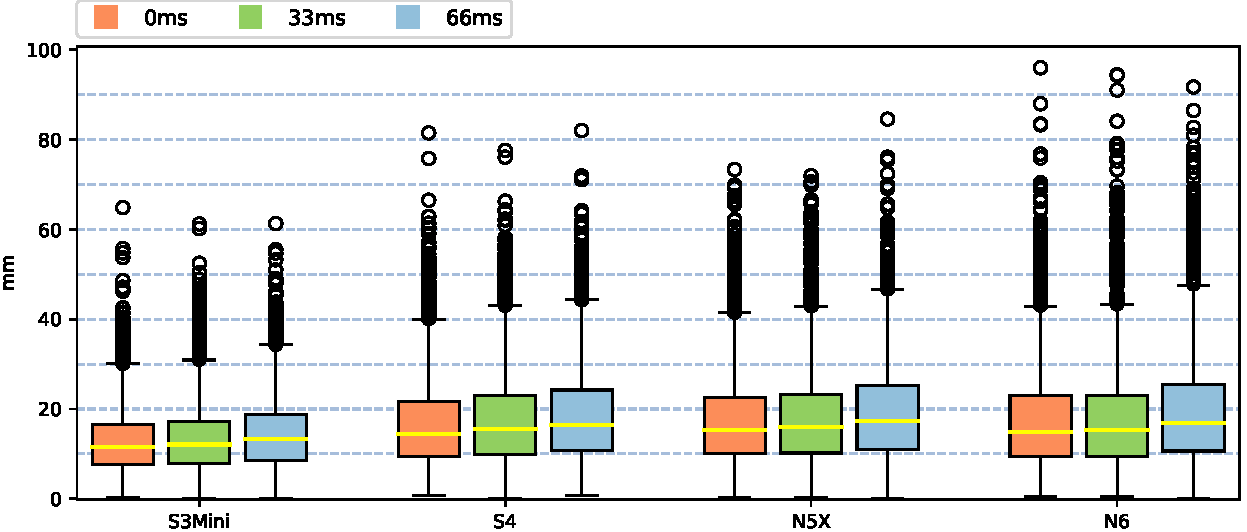
\includegraphics[width=\textwidth]{boxplot_general_smartphones}
	\caption{Boxplots for the predictions of the general model. The groups are based on the phones with each prediction time as one box.}
	\label{fig:boxplots_general}
\end{figure}
We trained our models for approximately 2000 epochs.
For each point prediction we converted its unit from pixels to mm based on the pixel sizes of the mobile phones.
The average euclidean distances for both the single and the general model can be seen in \cref{tab:results}.
\cref{fig:boxplots_general} visualizes the errors of the general model grouped by phones for each prediction time.
\todo{Maybe noch ein origin plot wenn platz}
For \cref{fig:ell_single} and \cref{fig:ell_general} we have shifted each prediction with its corresponding true point by the distance from the true point to the origin, thus resulting in a heatmap around the origin representing the scattering of the prediction points.
For each phone and each prediction time we have fitted an elliptic envelope with a contamination of .0261 inside the heatmap.
Elliptic envelopes are used for outlier filtering; the higher to contamination the more aggressive the ellipse is fitted against outliers.
For each ellipse of single and general models we calculated the area in $ mm^{2}$.
The areas are listed in \cref{tab:areas}.
Light green highlighted cells depict which model resulted in a smaller ellipse area for its predictions.
%\footnote{\url{https://05.jupyter.interactionlab.io/user/beneste/tree/fapra-imu}}
